\documentclass[border=2pt]{standalone}
\usepackage{tikz}
\usetikzlibrary{arrows.meta,chains}

\begin{document}
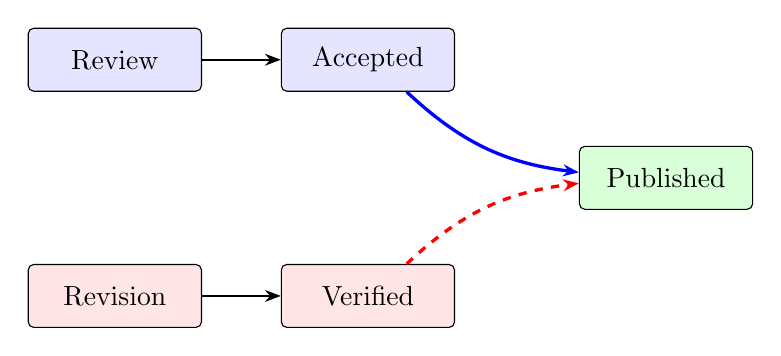
\begin{tikzpicture}[
  start chain=approved going right,
  start chain=rejected going right,
  start chain=release going right,
  stage/.style={
    draw,
    rounded corners=2pt,
    minimum width=22mm,
    minimum height=8mm,
    align=center
  },
  every join/.style={-{Stealth[length=2mm]},very thick}
]
  \node[stage,on chain=approved,fill=blue!10] (review) at (0,1.5) {Review};
  \node[stage,on chain=approved,fill=blue!10] (accepted) {Accepted};

  \node[stage,on chain=rejected,fill=red!10] (revision) at (0,-1.5) {Revision};
  \node[stage,on chain=rejected,fill=red!10] (verified) {Verified};

  \node[
    stage,
    on chain=release,
    fill=green!15,
    join=with approved-end by {blue,bend right=18},
    join=with rejected-end by {red,dashed,bend left=18}
  ] (published) at (7,0) {Published};

  \path[-{Stealth[length=2mm]},thick]
    (review) edge (accepted)
    (revision) edge (verified);
\end{tikzpicture}
\end{document}
